% LTex: language=pl
\chapter{Wdrożenie}

% --------------
% Serwer fizyczny
% -------------

\section{Serwer fizyczny}
W ramach przebudowy istniejącego systemu STOS zostały zakupione 2 nowe serwery fizyczne w ramach przetargu rozpisanego przez Politechnikę Gdańską, na które miał zostać wdrożony system STOS.

\subsection{Komponenty serwera}
Każdy z tych serwerów zbudowany jest oparty na architekturze AMD64 i korzysta z chipsetu AMD X670 i gniazda procesora zgodnego ze specyfikacją AM5 oferowanych przez płytę główną GIGABYTE X670 Gaming v2 \cite{gigabyteX670}. Jako procesor wykorzystano kompatybilny z płytą główną procesor AMD Ryzen 9 7950X, posiadający 16 rdzeni i 32 wątki o bazowym taktowaniu zegara o częstotliwości $4,5 Ghz$ i taktowaniem maksymalnym $5,7 Ghz$ \cite{ryzen}. Wspiera on maksymalnie $128 GB$ pamięci RAM w standardzie DDR5, w tym serwerze zainstalowano zestaw 4 kości, każda o pojemności $32 GB$, składające się na zestaw Patriot Viper Venom 128GB DDR5, z taktowaniem $6400 Mhz$ i opóźnieniem CAS wynoszącym 32 cykle zegara (CL32) \cite{patriotRam}. Za chłodzenie procesora odpowiada chłodnica Shadow Rock 3 produkowana przez firmę CoolerMaster, wykorzystująca mechanizm chłodzenia powietrznego \cite{coolermaster}. Na pamięć trwałą serwera składają się 3 dyski, 2 dyski w technologii M.2 Samsung Evo 990 o pojemności $1 TB$ każdy \cite{samsungSsd}, i dysk SSD Silicon Ace A55 \cite{sataSsd} o pojemności $4 TB$, łącznie dające $6 TB$ pamięci trwałej. System zasilany jest zasilaczem Gigabyte UD1000GM PG5, certyfikowanym standardem 80+ Gold i charakteryzującym się dostarczaną mocą w wysokości $1 kW$ \cite{zasilka}.  Obudową serwera jest obudowa Silver Monkey X Fence SMXC008 z wbudowanym wentylatorem o średnicy 120 mm \cite{obudowa}.

\subsection{Potencjalne wady konfiguracji sprzętowej}
Pierwszym potencjalnym problemem wynikającym z powyższej specyfikacji sprzętowej jest ograniczenie możliwej do wykorzystania pamięci RAM narzucone przez procesor. W razie potrzeby zwiększenia dostępnej pamięci operacyjnej na serwerze konieczna jest również wymiana procesora na taką jednostkę, która pozwala na skorzystanie z takiej, większej, ilości pamięci. Kolejnym potencjalnym wąskim gardłem jest zastosowane rozwiązanie chłodzenia procesora. Chłodnica wykorzystana w serwerze, CoolerMaster Shadow Rock 3, według specyfikacji, jest w stanie skutecznie utrzymać akceptowalną temperaturę procesora o mocy do $190 W$, wyrażanej jako TDP (Thermal Design Power), oznaczająca maksymalne zużycie mocy przez komponent, w tym przypadku procesor, które należy brać pod uwagę przy projektowaniu systemu \cite{intelTdp}. AMD Ryzen 7950X, przy bazowym taktowaniu zegara, szacowany jest przez producenta na charakteryzujący się mocą $170 W$ TDP. Sam zapas $20W$ jest wystarczający w przypadku chłodzenia procesora, lecz w przypadku Ryzena 7950X pracującego w trybie boost, jego zużycie energii jest w stanie dochodzić do ok. $230 W$ - $250 W$ \cite{amdPpt, testyMocy}, co jest równoznaczne z deficytem mocy chłodnicy rzędu od $40W$ do $60W$. Zastosowanie obecnego chłodzenia może, z dużym prawdopodobieństwem, doprowadzić do powstania efektu znanego jako "thermal throttling" \cite{throttling}. Polega on na ograniczaniu mocy i prędkości procesora, gdy osiąga on temperatury dochodzące do maksymalnych dopuszczalnych przez producenta temperatur, mieszczących się zazwyczaj w zakresie od $95^{\circ}\mathrm{C}$ do $105^{\circ}\mathrm{C}$. W przypadku powyższej konfiguracji, efekt ten powstawać będzie przy zwiększonym obciążeniu serwera, uniemożliwiając procesorowi wykorzystanie w pełni jego potencjału taktowania. Dodatkowym czynnikiem jest stosunkowo niska objętość powietrza odprowadzanego ze środka obudowy serwera, za którą odpowiedzialny jest jeden wiatrak o średnicy 120 mm. Warto nadmienić, że są to jedynie rozważania teorytyczne i w celu ustalenia faktycznej wydajności zastosowanego chłodzenia, należałoby przeprowadzić odpowiednie testy serwera, które nie znajdują się w zakresie tego projektu.

\begin{figure}[!h]
	\begin{center}
		\resizebox{0.7\textwidth}{!} {
			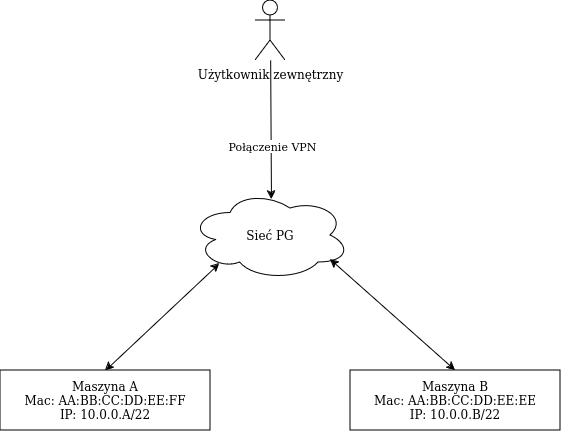
\includegraphics{img/4/fizycznaSiec.png}
		}
		\caption[Diagram fizycznego rozmieszczenia maszyn w sieci Politechniki Gdańskiej]{Diagram przedstawiający umiejscowienie maszyn fizycznych w sieci Politechniki Gdańskiej. Adresy IP i adresy MAC nie są faktycznymi adresami maszyn w sieci. Źródło własne.}
		\label{diagramSiecFizyczna}
	\end{center}
\end{figure}

\subsection{Serwery w kontekście sieci Politechniki Gdańskiej}
Obie maszyny fizyczne znajdują się na terenie Politechniki Gdańskiej i znajdują się w sieci wewnętrznej PG. Posiadają one statycznie przypisane z poziomu sieci adresy IP, odpowiadające adresom MAC ich kart sieciowych. Dostęp z sieci zewnętrznych odbywa się za pomocą VPN Politechniki Gdańskiej i uzyskaniu dostępu do sieci politechnicznej. Topologię maszyn fizycznych w kontekście sieci przedstawia diagram \ref{diagramSiecFizyczna}.


% --------------
% Kubernetes
% -------------

\section{Koncepcja wdrożenia jako klaster Kubernetes}
Aby efektywnie wykorzystać wcześniej wspomniane mechanizmy ograniczania wykorzystywanych zasobów sprzętowych, pierwsza koncepcja architektury wdrożenia systemu była oparta na orkiestratorze kontenerów Kubernetes, systemie pozwalającym na zautomatyzowane wdrażanie, skalowanie i zarządzanie potencjalnie wysoką liczbą kontenerów \cite{k8sMain}.

\subsection{Orkiestratory kontenerów}
Wraz ze wzrostem popularności architektur aplikacji opartych na mikroserwisach, wzrosła również podaż na systemy pozwalające na zarządzanie, monitorowanie i skalowanie instancji poszczególnych serwisów aplikacji wdrożonych na wielu maszynach fizycznych, szczególnie w dużych systemach komercyjnych. Odpowiedzią rynku wypełniającą tę lukę są systemy orkiestracji kontenerów. Dwoma najpopularniejszymi orkiestratorami na rynku są Kubernetes i Docker Swarm.

\subsubsection{Docker Swarm}
Docker Swarm to rozwiązanie wbudowane bezpośrednio w silnik Dockera, pozwalające na stosunkowo proste wdrożenie złożonych aplikacji \cite{dockerSwarm}. Zawiera podstawowe funkcjonalności orkiestratora, takie jak wdrażanie aplikacji za pomocą plików konfiguracyjnych (korzysta ze standardu Docker Compose \cite{dockerCompose}), monitorowanie stanu serwisów oraz obsługę wdrożenia na kilku maszynach fizycznych. Niewątpliwą zaletą tego rozwiązania jest jego prostota i stosunkowo niski próg wejścia dla użytkowników zaznajomionych z technologią Docker i Docker Compose, co pozwala na uniknięcie kosztów związanych ze szkoleniem administratora systemu. Jednakże prostota ta wiąże się również z ograniczeniem możliwości konfiguracji takiego systemu, a dość niska popularność Docker Swarm w porównaniu do Kubernetes niesie za sobą koszty związane z samodzielną implementacją pewnych rozwiązań, których odpowiedniki w technologii Kubernetes są dostępne za darmo i utrzymywane przez społeczność.
\subsubsection{Kubernetes}
Kubernetes to rozwiązanie, z którego korzystają największe projekty komercyjne \cite{googleKubernetes}, początkowo rozwijane przez firmę Google. Sam system Kubernetes dostępny jest, podobnie jak system operacyjny Linux, w postaci różnych dystrybucji. Spółki oferujące usługi chmurowe dla klientów, takie jak Amazon i Google, często decydują się na rozwój własnych dystrybucji Kubernetesa, lecz istnieją również dystrybucje przeznaczone dla mniejszych projektów, takie jak MicroKubernetes \cite{microk8s}, który został wykorzystany podczas prototypowania rozwiązania wdrożenia systemu STOS. Kubernetes posiada bogaty ekosystem i wbudowane rozwiązania, pozwalające na znaczące uproszczenie konfiguracji wirtualnej sieci, w której znajduje się wdrażany system. Rozwiązanie to, w przeciwieństwie do Docker Swarm, jest niezależne od zastosowanej technologii konteneryzacji, pozwalając na używanie więcej niż jednej technologii w ramach jednego klastra. Dodatkowo Kubernetes wspiera menadżera pakietów/zasobów w postaci programu Helm \cite{k8sHelm}, dzięki czemu dostępnych jest wiele darmowych rozwiązań utrzymywanych przez społeczność, pozwalających między innymi na automatyczne gromadzenie logów i monitorowanie poszczególnych serwisów wdrożonych w systemie. Podobnie jak w przypadku Docker Swarm, stopień skomplikowania Kubernetesa stanowi jego największą zaletę i wadę. Przez wysoki próg wejścia, administracja systemem, a w szczególności jej nauka, stanowi czasochłonny proces. Podobnie jest w przypadku utrzymania, dla osób niezaznajomionych z Kubernetesem i jego poszczególnymi elementami, diagnostyka potencjalnych problemów i ich naprawa staje się nieporównywalnie trudniejszym zadaniem niż w przypadku Docker Swarm. Jednakże, rozwiązanie wdrożone na bazie klastra Kubernetes oferuje o wiele więcej możliwości potencjalnego rozwoju systemu, zarówno pod względem bardziej rozbudowanej architektury, jak i wdrażania dodatkowych rozwiązań monitorowania.

\subsection{Wybór orkiestratora}
Mając na uwadze wady i zalety rozwiązań opartych o MicroKubernetes i Docker Swarm, podjęto decyzję o początkowym rozwoju rozwiązań opartych o obie z tych technologii. Faktycznie, wdrożenie samej aplikacji za pomocą Docker Swarm zajęło zauważalnie mniej czasu niż w przypadku MicroKubernetesa (osoba wdrażająca nie miała wcześniejszego doświadczenia z żadnym z tych systemów). Przy próbie wdrożenia rozwiązania pozwalającego na monitorowanie logów systemu, prawidłowość ta prezentowała się zgoła odwrotnie - dzięki menadżerowi pakietów Helm, wdrożenie tzw. "stacka ELK" (czyli aplikacji Elasticsearch, Logstash i Kibana) na klastrze MicroKubernetes odbyło się nieporównywalnie szybciej niż w przypadku Docker Swarm, który wymagał ręcznej konfiguracji poszczególnych kontenerów odpowiedzialnych za każdy z serwisów wchodzących w skład rozwiązania zbierającego logi z systemu. Na podstawie doświadczeń związanych z utrudnionym wdrożeniem zewnętrznych systemów na klastrze Docker Swarm i możliwych przyszłych komplikacjach przy konieczności dodawania kolejnych serwisów do klastra, podjęto decyzję o kontynuowaniu prac z MicroKubernetesem.

\subsection{Prototyp wdrożenia i jego zalety}
Z perspektywy administratorów systemu STOS i pracowników katedry, którzy w przyszłoći będą utrzymywać i rozwijać system STOS, główną zaletą podejścia opartego o technologię orkiestracji kontenerów, w słowach inżynierów firmy Google \cite{googleKubernetes}, jest przeniesienie wielu odpowiedzialności ze środowiska, w którym działa aplikacja, na samą aplikację. Pozwala to na uniezależnienie obecnych i przyszłych komponentów systemu STOS od środowiska, w którym zostały wdrożone, co znacząco ułatwia prowadzącym lub studentom rozwijającym i utrzymującym system STOS na dodawanie, lub modyfikowanie jego funkcjonalności. Ponadto Kubernetes zawiera wbudowane funkcjonalności monitorowania zużycia zasobów systemowych i umożliwia konfigurację automatycznego ponownego uruchamiania aplikacji po wystąpieniu błędu \cite{k8sPod}.

\begin{figure}[!h]
	\begin{center}
		\resizebox{0.7\textwidth}{!} {
			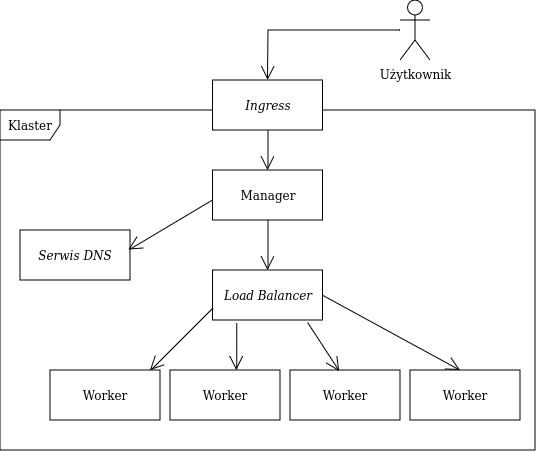
\includegraphics{img/4/k8s.png}
		}
		\caption[Diagram prototypu klastra Kubernetes]{Diagram przedstawiający elementy prototypu klastra Kubernetes wdrożonego dla systemu STOS. Źródło własne.}
		\label{diagramk8s}
	\end{center}
\end{figure}

W ramach projektu inżynierskiego powstał prototyp takiego klastra, zawierający symulowaną architekturę systemu STOS (\ref{diagramk8s}). Umożliwiał on dynamiczne skalowanie ilości instancji serwisu "worker", odpowiedzialnego za ewaluację zadań przesyłanych przez studentów, jak i monitorowanie stanu wszystkich działających w ramach systemu usług.

Oprócz samych komponentów systemowych STOSu zaprojektowany klaster oferował również szereg usług dodatkowych. Jedną z nich jest wbudowany serwer DNS, który znacząco ułatwia konfigurację komunikacji pomiędzy usługami systemu \cite{k8sDns}. Drugim najważniejszym komponentem był "service" w kontekście Kubernetesa, pełniący funkcję load-balancera dla poszczególnych serwisów "worker". Tym sposobem, zagwarantowano równomierne obciążenie każdej instancji serwisu, bez względu na ilość działających kontenerów \cite{k8sService}. Ostatnim z elementów klastra była usługa Ingress, pozwalająca na jednoznaczne zdefiniowane punktu dostępu do serwisów klastra ze środowiska zewnętrznego, którym w tym prototypie był serwis "manager" \cite{k8sIngress}.

\subsection{Koncepcja wdrożenia a dynamika wymagań}
Jednakże, w trakcie prac i w kontekście dynamicznie zmieniających się wymagań, wdrożenie systemu STOS jako klaster oparty na orkiestratorze kontenerów okazało się przedsięwzięciem bardziej skomplikowanym, niż mogłoby się to wydawać na początku prac. Wymaganiem była możliwość kontrolowania kontenerów Docker z poziomu samej aplikacji, będącej częścią STOSu. Łączyło się ono z większym stopniem złożoności rozwiązania spowodowanej wprowadzeniem dodatkowych komponentów lub zastosowaniem zaawansowanych wzorców projektowych przeznaczonych dla skonteneryzowanych aplikacji rozproszonych, takich jak "sidecar pattern" \cite{k8sPatterns}. Projekt rozwiązania opierającego się na klastrze Kubernetes i korzystający z dodatkowych komponentów systemowych przedstawiono na rysunku \ref{diagramk8sFinal}.

\begin{figure}[!h]
	\begin{center}
		\resizebox{0.7\textwidth}{!} {
			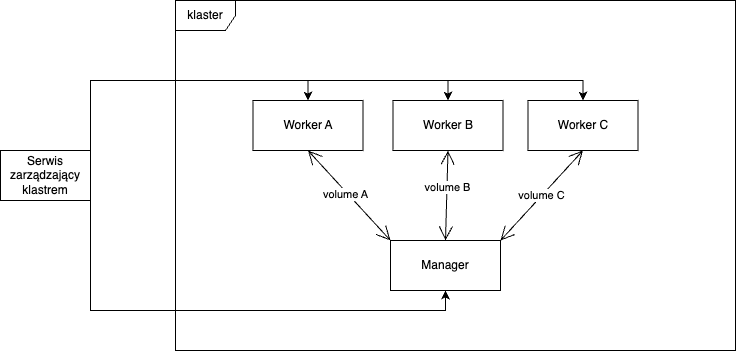
\includegraphics{img/4/k8sFinal.png}
		}
		\caption[Diagram prototypu klastra Kubernetes po zmianie architektury]{Diagram przedstawiający ogólną architekturę systemu wdrożonego na klaster Kubernetes po zmianie wymagań dotyczących konteneryzacji serwisu "worker". Źródło własne.}
		\label{diagramk8sFinal}
	\end{center}
\end{figure}

Zgodnie z wymaganiami, których źródłem są istniejące komponenty systemu STOS, komunikacja między kontenerem "worker" i serwisem "manager" musi być zrealizowana za pomocą współdzielonych katalogów. Taki mechanizm oferowany jest zarówno w postaci wolumenów w Dockerze \cite{dockerVolume}, jak i StatefulSet w Kubernetes \cite{k8sStateful}. Za zlecanie ewaluacji zadania i dynamiczne uruchamianie serwisu "worker", w tym modelu systemu odpowiedzialny jest dedykowany serwis uruchomiony poza klastrem, posiadający pełny dostęp do mechanizmów zarządzania tym klastrem.

Dodanie serwisu, którego awaria wiąże się z awarią całego systemu w postaci zewnętrznego serwisu nadzorującego stan klastra i cykl życia kontenerów to tylko część wad tego rozwiązania. Przy zastosowaniu kontenerów, które muszą utrzymywać swój stan, czyli skorzystaniu z technologii StatefulSet, dodatkowym czynnikiem przyczyniającym się do skomplikowania aplikacji jest zarządzanie współdzielonymi wolumenami, z których korzysta serwis "manager" w celu komunikacji z instancjami serwisu "worker". Dodatkowo niemożliwe staje się zastosowanie wbudowanego w klaster Kubernetes serwisu odgrywającego rolę "load-balancera", co wiąże się z koniecznością ręcznej implementacji tej funkcjonalności.

Z racji rosnącego stopnia skomplikowania wdrożenia systemu STOS za pomocą klastra Kubernetes, podjęta została decyzja o zaprojektowaniu rozwiązania nieopierającego się na technologii orkiestracji kontenerów.
